\chapter{Goal-oriented PMC for Reliability Analysis of Self-adaptive Systems}\label{ch:proposal}

This chapter presents our proposal for goal-oriented dependability analysis applied to the MPERS case study. Both TROPOS early and late requirements analysis phases are presented, as well as the goal-oriented probabilistic verification that requires a goal model with additional runtime regex for behaviour specification (RGM) and the context notations specifying context effects (CGM).

%Further details about the TROPOS methodology may be found in the reference literature~\cite{Bresciani:2004}. 


%from a goal model alternative selected for analysis of a given local or root goal 

Figure~\ref{fig:CRGM_TO_DTMC} illustrates the goal-oriented reliability analysis process that starts with conventional goal-oriented modelling and analysis phases of the TROPOS methodology and finishes with the generation of a high-level DTMC model used for reliability analysis. 

%Figure~\ref{fig:GODA_MODELS} presents the models involved in the analysis.

\begin{figure*}[h!]
\centering
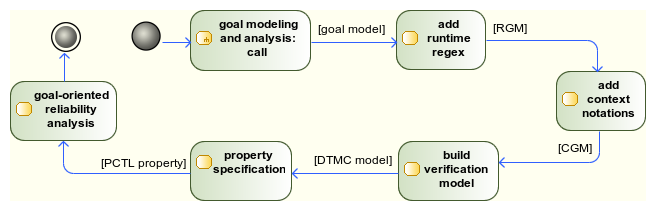
\includegraphics[width=0.9\textwidth]{imgs/CRGM_TO_DTMC.png}
\caption{Goal-oriented dependability analysis activities.}
\label{fig:CRGM_TO_DTMC}
\end{figure*}

The next sections are structured as follows. First, a goal modelling and analysis as described by TROPOS methodology is performed~\cite{Bresciani:2004}. Next, the RGM behaviour rules are further explained and added to the MPERS goal model. Then, context notation is added to the RGM. After this, the high-level DTMC model for MPERS is built and details about the mapping of a RGM into a DTMC in PRISM language are provided, as well as the inclusion of the CGM context effects. Next, PCTL properties representing the reliability of fulfilling different system goals are defined. Finally, we demonstrate how our verification approach may be employed in reliability analysis. 


\section{Mobile Personal Emergency Response System}

The MPERS case study will be further detailed in later sections as the proposed goal-oriented reliability analysis based on PMC is described using the MPERS goal models created at the requirements engineering phases of TROPOS methodology. As such, this section will be limited to cover some relevant aspects of this system that justify the use of our formal verification approach to analyse its reliability.

An emergency response system is a mission-critical system for which failures in achieving its main goals by the time they are required may lead to catastrophic consequences on users, i.e., on individuals monitored by the system expecting to be promptly assisted in case of a medical emergency. Accordingly, any stakeholder that wishes to offer a service based on this system will have both ethical and contractual obligations regarding the safety of its product, that is, it must employ all means to prevent system failures and to attain dependability.

MPERS is expected to have a high availability - as it must be ready to respond to an emergency that may happen at any time - and a high reliability - as an incorrect emergency response may lead to death or to costly false-positives. Integrity is a less critical attribute in this case, but it must also be addressed as user's privacy may not be violated by disclosing his personal health or geolocation information to unauthorized persons. Maintainability is addressed, among others, by the use of a software development methodology and by the ability to update emergency rules remotely at runtime.

Environment changes is an important factor for MPERS, as the following conditions may change:

\begin{itemize}

\item The battery of the mobile device;
\medskip

\item The battery of the vital signs sensors;
\medskip

\item The disc memory used for storing the vital signs history;

\item The mobile signal used for data communication and for geolocation triangulation;
\medskip

\item The GPS signal used for geolocation;
\medskip

\item The health risk of the patient;
\medskip

\end{itemize}



%TODO: IN CONTEXT SECTION
%For all these environment variables, a context analysis as proposed by Ali et al. may be employed for the creation of the rationale for context monitoring, i.e., for how each context condition may be asserted as true or false through the monitoring of environment information. Some contexts are mapped to single monitorable facts, like `GPS signal' and `battery life'. Other like `patient health risk' are composed of multiple facts in a propositional formula.


%Reliability verification of an Ambient Assisted Living System also based on body-area networks though PCM technique was explored by Fernandes~[Fernandes, 2012]. Reliability estimation demonstrates the non-determinism in the verification model that will result in an non-deterministic evaluation result. Moreover, PRISM cost/reward structures could be used for the verification of non-functional metrics such as power consumption. In this work, we limit the analysis to the reliability verification as part of a dependability analysis.

%It will be up to the analyst and stakeholders to define which type of probabilistic model and which PCTL properties must be analysed for each different system. Dependability attributes may be relevant for any sort of system, but are certainly important for systems with some criticality degree, i.e., for those whose failure could have severe or catastrophic consequences for the user(s) and for the environment.



\section{Goal Modelling and Analysis}

The goal modelling and analysis of both early and late requirements phases in TROPOS methodology are applied to our MPERS case study. Next subsections briefly describe these two phases and present the resulting models.

\subsection{TROPOS Early Requirements Phase}

In early requirements phase, stakeholders and their needs are modelled in a goal model diagram. Each actor may be a depender or a dependee of a goal, task or resource dependency. In this phase, only social dependencies to the system actor and between application domain stakeholders are analysed, leaving the detailed system analysis to later development phases.

\begin{figure*}[ht!]
\centering
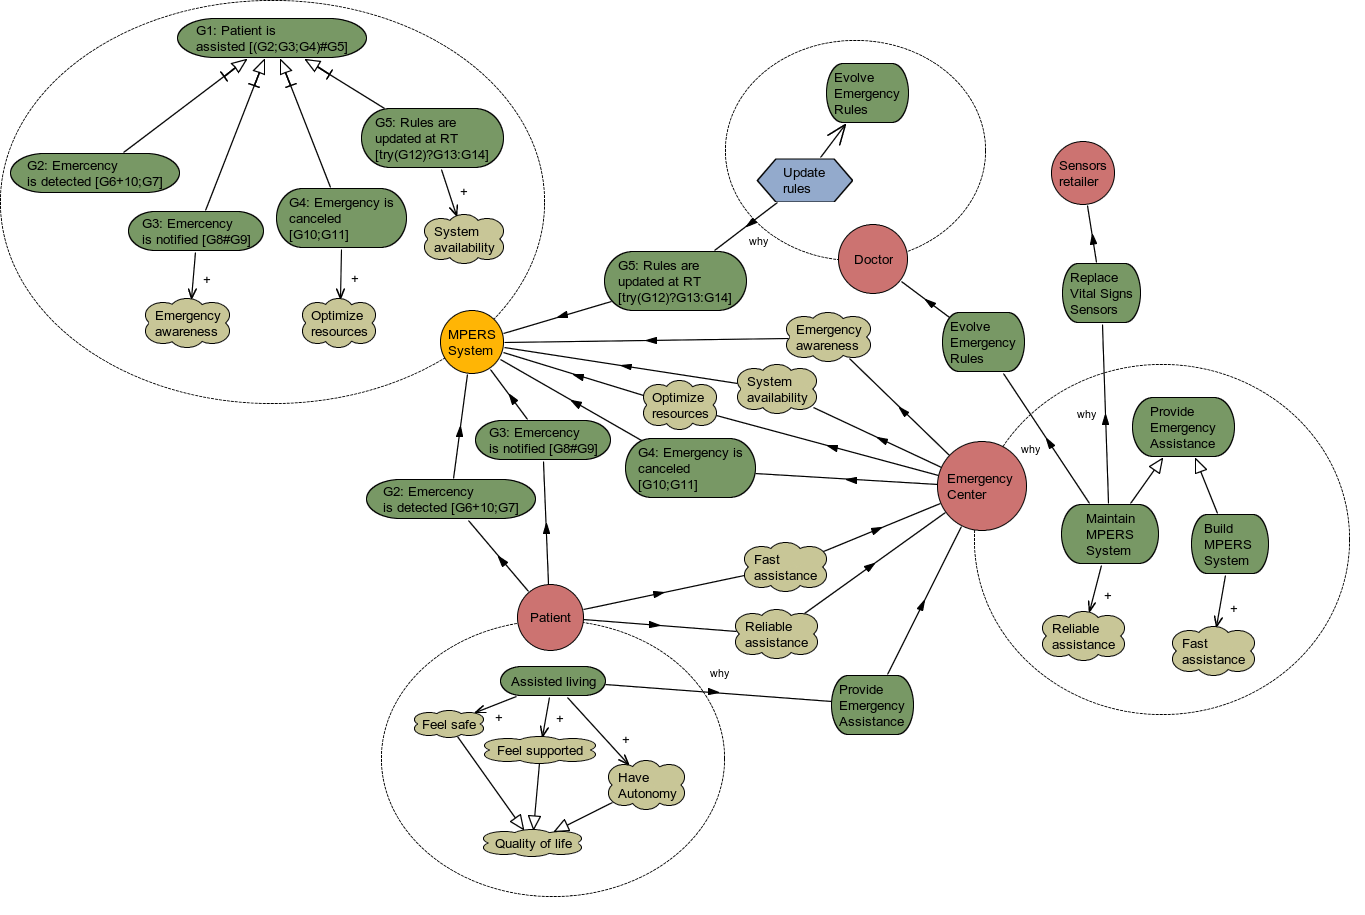
\includegraphics[width=1\textwidth]{imgs/MPERS_ER.png}
\caption{MPERS at TROPOS early requirements phase}
\label{fig:MPERS_ER}
\end{figure*}

The MPERS sytem and its social dependencies are presented by the actor model in Figure~\ref{fig:MPERS_ER}. System actors and social actors are displayed in different colors. Among the stakeholders, the emergency center represents a private or public organization interested in providing an emergency response service to patients. Patient and doctor represent, respectively, the assisted person and the medical responsible for defining and evolving the emergency detection rules as part of an evolutionary approach for personal emergency response. Finally, sensors retailer should provide the vital signs sensors required for monitoring.

From the diagram in Figure~\ref{fig:MPERS_ER} it is possible to have a first look of the MPERS system-to-be. Main goals are divided in detecting, notifying and checking an emergency. Also, the ability to update the emergency rules at runtime (RT) is the fourth and last mandatory goal (AND-decomposition) that fulfils the `Patient is assisted' root goal. System goals and softgoals are directly or indirectly related to stakeholders needs.

The distinguished yellow circle indicates that MPERS is a system actor. MPERS goals can be seen with a regex indicating its dynamic behaviour as part of the runtime goal model specification required by the proposal. This notation is a reflex of the late requirements phase, as the TAOM4E tool used for goal modelling shares unique entities and relations among different development phases. The regex syntax is enclosed by brackets to differentiate then from goal name. More details on the behaviour specification can be found in later section of this chapter.

%In future work, a specific modelling compartment should receive the values for the runtime regex.

\subsection{TROPOS Late Requirements Phase}

\begin{figure*}[h!]
\centering
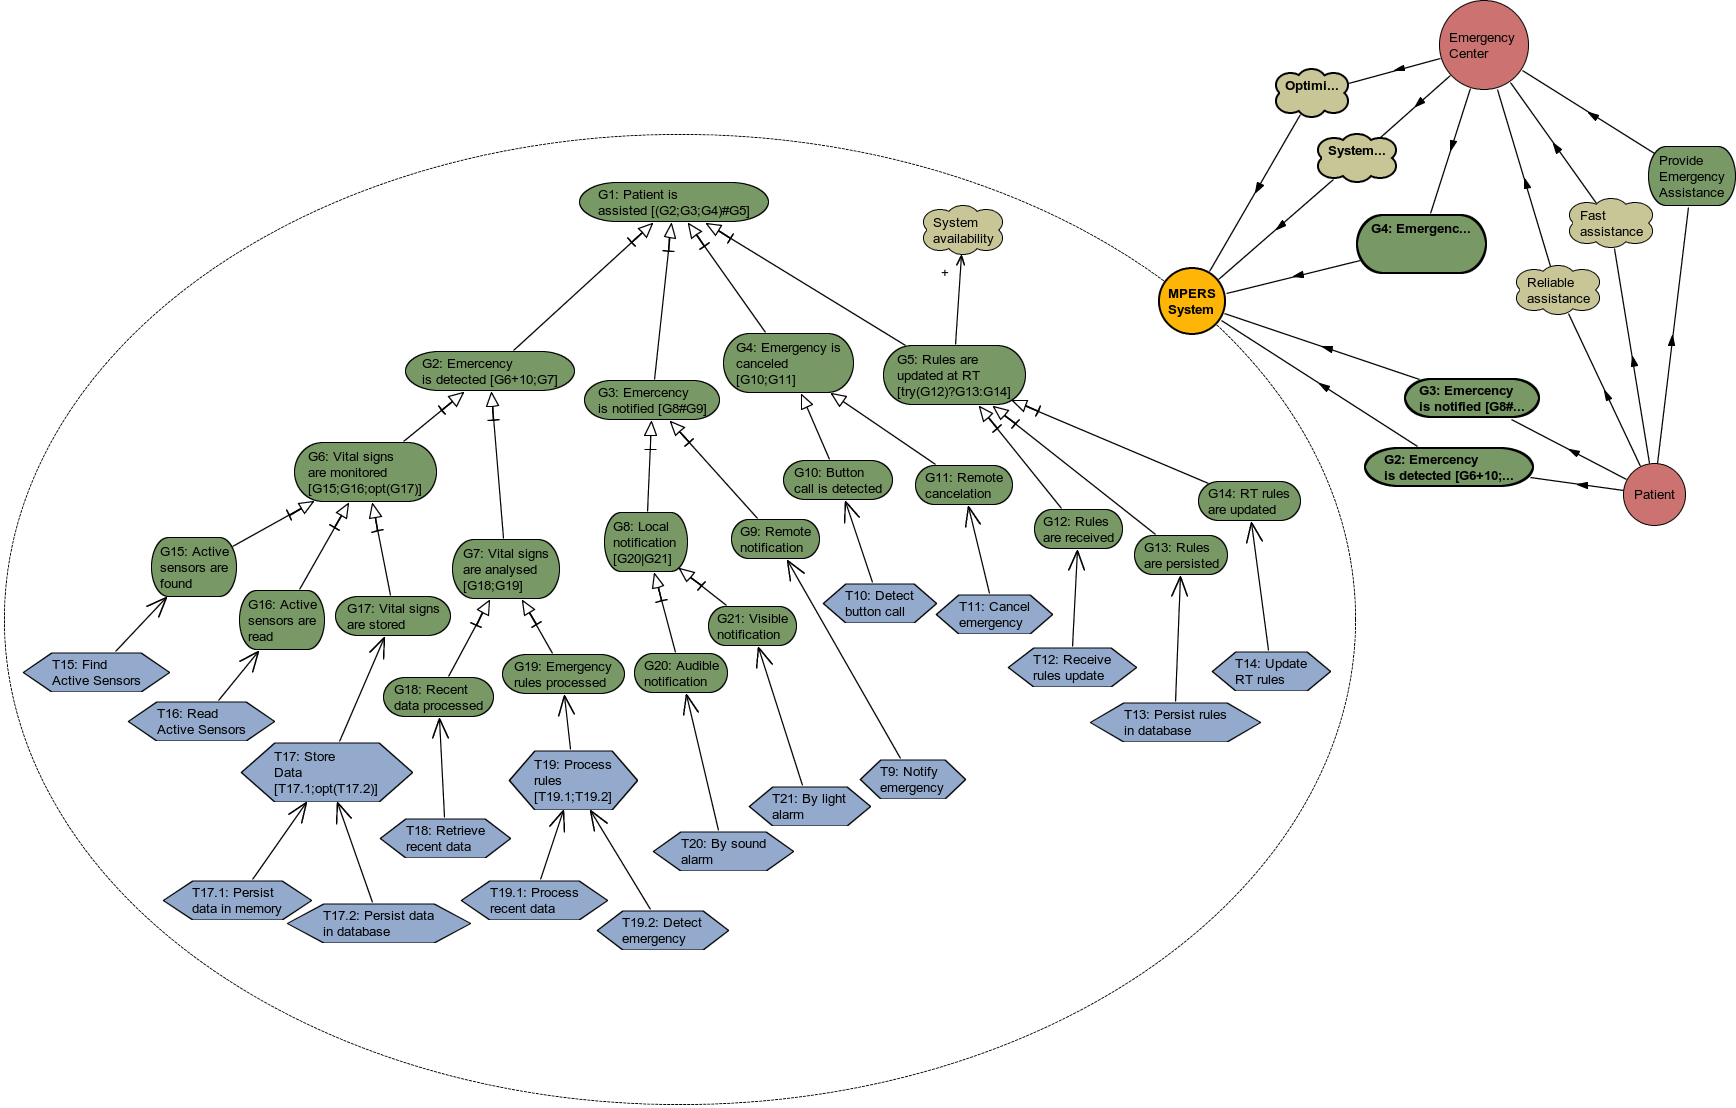
\includegraphics[width=1\textwidth]{imgs/MPERS_LR.png}
\caption{MPERS at TROPOS early requirements phase}
\label{fig:MPERS_LR}
\end{figure*}


Later requirements phase concentrates the analysis in the system-to-be and its operational environment. The MPERS goal model occupies the most part of the diagram and each of its main goals are further decomposed through AND/OR decomposition. Also, means-end tasks specifies how leaf-goals can/must be fulfilled and the runtime regex across goals and tasks specifies dynamic properties of the system-to-be behaviour. Figure~\ref{fig:MPERS_LR} illustrates the late requirements diagram for the MPERS.

At this stage of the methodology, the system is represented as a monolithic actor and its goal model may be extended with the runtime specification. This extended model merges multiple views in the same diagram: goals, tasks and relations represent the requirements view for the system-to-be as well as the intentionality behind then, while the runtime specification provides the behaviour specification required for our goal-oriented dependability analysis. 

%in terms of goal achievement  and task execution.

%REVISE
To evaluate our proposal, we have explored the use of the PMC technique for the reliability verification of the system goal model resulting from the TROPOS late requirements phase. The idea is to initially evaluate the approach in a monolithic representation without the additional complexity of a multi-agent architecture. The evaluation involving later TROPOS phases should be explored in future work. The remaining of this section will focus on the proposed goal-oriented contextual dependability analysis.

\subsection{RGM - UML activity diagram comparison}\label{ssec:RGM-UML}

A similar behaviour specification achieved with the RGM in Figure~\ref{fig:MPERS_LR} could be provided by an UML activity diagram with activities representing the leaf-tasks in the model. However, activity diagrams have an homogeneous abstraction level and do not clearly correlate behaviour to the requirements they are meant to satisfy. In contrast to the RGM, activity diagrams denote behaviour through graphical symbols, while the RGM mixes the original goal model notation with a runtime regex. This simple notation increases the utility of a goal model diagram. Figure~\ref{fig:MPERS_UMLAD} presents an activity diagram corresponding to the MPERS leaf-tasks. 

\begin{figure*}[h!]
\centering
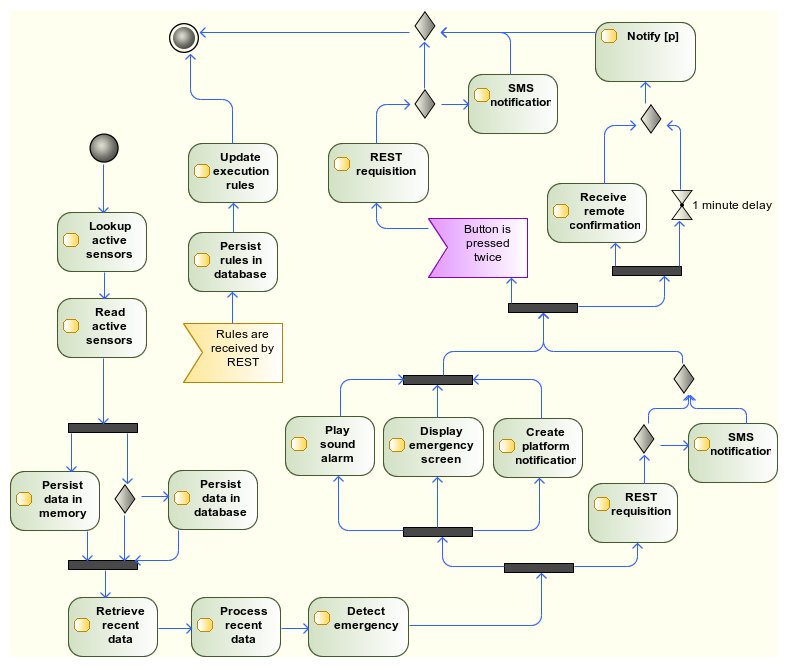
\includegraphics[width=1\textwidth]{imgs/MPERS_UMLAD.png}
\caption{MPERS tasks represented by a UML activity diagram}
\label{fig:MPERS_UMLAD}
\end{figure*}

Among its limitations, RGM does not express that an emergency has to be confirmed after a time (clock) or signal event as the UML activity diagram does. Both necessary and sufficient conditions for the triggering and fulfilment of goals, tasks and dependencies are provided by Formal TROPOS specification language.  Still, sequential, interleaved, alternative, optional and conditional execution flows as well as multiple executions of the same task can be expressed by the RGM, providing a rich behaviour specification for the system-to-be.

%could be checked for non-functional requirements such as dependability attributes.

The idea of a runtime goal model is not to replace UML activity diagrams, but to complement the static goal model with a clear runtime syntax that could be used for 
documentation, team communication and for conformance verification at both design time - e.g., through model-based verification - and during system execution - as the execution monitoring originally proposed by Dalpiaz et al~[RGM]. Depending on the complexity of the behaviour specification, a more robust runtime syntax would have to be employed or complemented by traditional UML behaviour models. In this work, RGM is used as input for our goal-oriented dependability analysis based on PMC.


%\section{Goal-oriented contextual dependability analysis}

%To evaluate our verification approach with the MPERS case study, we have used a discrete-time Markov chain (DTMC) probabilistic model and focused on the verification of NFR related to dependability, i.e., NFR that are either direct attributes encompassed by dependability or that are related to one or more of these attributes.

\subsection{Non-functional requirements analysis}

%\subsubsection{NFR framework with quantitative constraints}

TROPOS goal model also provides rationale for NFR analysis, as it originally inherited the softgoal analysis from the NFR framework~[NFR]. In our approach, non-functional constraints are modelled as qualitative hard goals with a clear cut value for its satisfaction, complementing the other NFRs modelled as softgoals. As a benefit of a goal-oriented modelling for NFRs, the elicitation of a given NFR may be justified by its relation to other elements in the model. Figure~\ref{fig:MPERS_NFR} presents the NFRs for the MPERS system actor.

\begin{figure*}[h!]
\centering
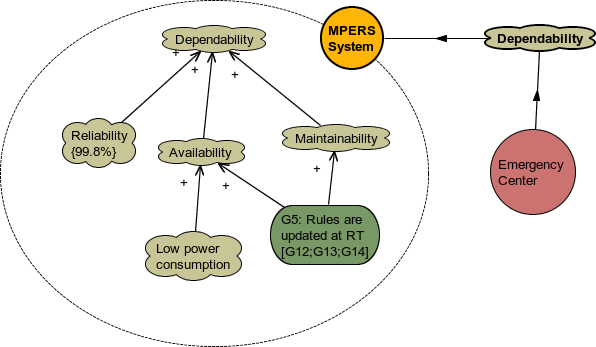
\includegraphics[width=1\textwidth]{imgs/MPERS_NFR.png}
\caption{MPERS non-functional requirements.}
\label{fig:MPERS_NFR}
\end{figure*}

%Intersting for motivation!
Similarly to the Awareness Requirements by Souza et al.~\cite{Souza:2011}, some NFR define metrics over other requirements. These meta-requirements are not directly fulfilled by system functionalities like `emergency awareness' is fulfilled by `notify emergency' or `confidentiality' could be fulfilled by `user authentication', but by how these functionalities will perform. Reliability, for instance, is inversely proportional to the likelihood of failures. Hence, the reliability metric depends on the probability of system functionalities to successfully meeting their goals. 

Other MPERS NFR are `emergency awareness' and `resources optimization'. These softgoals are addressed by system functionalities. The former receives a full contribution (double positive sign) from goal `emergency is notified', meaning it is fully satisfied by this goal. The later is just assumed to be partially satisfied by the `emergency is checked' functional goal.


%The conformity to these NFR is not implicit in the model, it requires some verification technique.

%PUT a goal model with hard goal NFRs!

%PUT SOME NFR CONCEPTUAL MODEL HERE!

Each requirement in a goal model must come from another requirement through decomposition, means-end or contribution links, or it must be directly mapped to stakeholder needs through dependency links. Emergency center attended the patient's needs by providing and maintaining the MPERS system itself and by assuring other NFR for the system. 

Reliability was selected as metric over the system execution (meta-requirement), while availability and maintainability are partially satisfied by the `low power consumption' softgoal and MPERS ability to update emergency rules at runtime, respectively. This proposal focus on reliability analysis and will not discuss the verification of other relevant NFRs.

%evaluation will focus on the reliability metric and, for the sake of simplicity, will omit the verification of other relevant NFRs.

\section{Goal-oriented Probabilistic Verification Model}\label{ssec:NFR-verification}

%NOT HERE!
%The probabilistic verification of systems with variability is not a novelty by itself. Many proposals have addressed this problem in the context of Dynamic Software Product Lines (DSPL), some of then using the PMC technique~[Vini, Paula, Who Else?]. In DSPL, optional and alternative features may be activated or deactivated at runtime. A family based verification of one or multiple NFRs, also called qualitative goals, indicates what combinations are valid or which combination is optimal.

This section describes the application of a goal-oriented PMC technique for the reliability verification of a runtime goal model with additional context effect notations. We call it a goal-oriented probabilistic verification or goal-oriented dependability analysis because the probabilistic model, in this case a DTMC model, is built directly from a runtime goal model with the purpose of evaluating PCTL properties related to the reliability of the system, i.e., to the success probability of different goals in being fulfilled.

% to verify the conformance of the RGM to defined non-functional constraints and also to solve the variability problem at design time considering both cases explained in Section~\ref{sec:variability}, i.e., for static context and dynamic contexts.

\subsection{Leaf-tasks as DTMC modules}


The MPERS RGM in Figure~\ref{fig:MPERS_LR} expands its main goals in further subgoals that are ultimately satisfied by operational tasks. Tasks can also be expanded in more granular subtasks. Tasks without outgoing relations are named leaf-tasks. In our proposal, leaf-tasks are mapped to modules in a DTMC model in PRISM language. In the DTMC model, leaf-tasks have their execution state mapped to a module variable (sT15 variable in Figure~\ref{fig:PRISM_TSK_MODULE}). From the RGM original set of goal/tasks instance states, we considered the following values:

\begin{itemize}

\item Init(sTask=0): corresponds to the initial/ready state of a given leaf-task. From this state, a transition may occur to the running state, if this task is part of a system alternative to be analysed, or directly to the final success state, if the opposite.
\medskip

\item Running(sTask=1): corresponds to the execution state of a given leaf-task. From this state, a transition to the final success or failure states may occur. A variable ranging from 0 - 1 defines the task's reliability, i.e., the probability of a transition to the success state - and the complementary transition probability to the failure state (variable rTask15 in Figure~\ref{fig:PRISM_TSK_MODULE}).
\medskip

\item Success(sTask=2): corresponds to the absorbing and final success state of a singular task execution.
\medskip

\item Skipped(sTask=3): indicates that a task does not participate in the fulfilment of the analysed goal and should not impact the analysis results.
\medskip

\item Failure(sTask=4): the opposite from the final success state, meaning that a singular task execution has failed.

\end{itemize}

Figure~\ref{fig:UML_TSK_STATES} illustrate leaf-tasks' states in a UML state diagram, while Figure~\ref{fig:PRISM_TSK_MODULE} presents a system task as a PRISM module.

\begin{figure*}[ht]
\centering
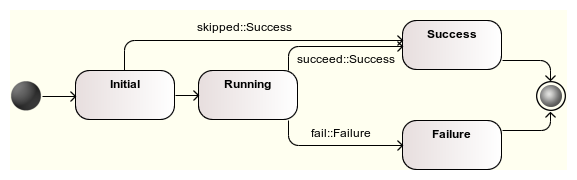
\includegraphics[width=0.8\textwidth]{imgs/UML_TSK_STATES.png}
\caption{State diagram for leaf-tasks in the DTMC module.}
\label{fig:UML_TSK_STATES}
\end{figure*}

%PRISM modules are containers for variables and commands, i.e., for states and behaviour

\begin{figure*}[ht]
\centering
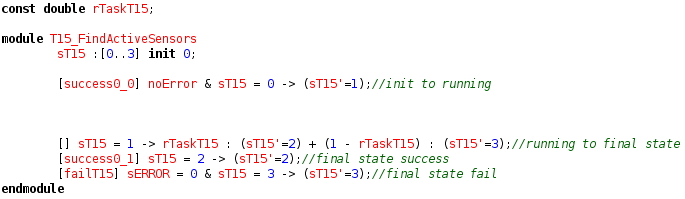
\includegraphics[width=1\textwidth]{imgs/PRISM_TSK_MODULE.png}
\caption{A PRISM DTMC module representing T15 (mandatory) task.}
\label{fig:PRISM_TSK_MODULE}
\end{figure*}


%init (0), running (1), success (2) and failure (3). Success and failure are the final absorbing states for a task instance. Transition to these states is conditioned to the rTask probability: the closer this variable is to 1, the higher the probability of reaching the success state. 


\subsection{Building the high-level DTMC model from a RGM}

%The state-based verification of non-functional constraints that specifies how different functionalities should perform is a complex task that involves a representation of system states and their transitions. A goal model may define system requirements with variable abstraction levels. As such, the feasibility of the verification of a given metric depends on the information provided by the model.

The first step in building a DTMC from a RGM is parsing the behaviour rules. All goals and tasks elements in the model receive an unique identification (ID). Numeric IDs are prefixed with an `G', in the case of goals, and `T', in the case of tasks. For each decomposed element, a corresponding runtime regex consisting of IDs and rules specifying the behaviour of all immediately underlying goals and tasks. Parenthesis are used for grouping related goals/tasks and for clarification purpose only, as temporal order is parsed from the type of the rule and its position in the regex.

%In the DTMC models for PMC verification of system behaviour, activities have their execution time mapped to discrete values. For instance, in a system workflow, initial activities start at a given time slot, e.g., zero. Considering the the following activities to only start after all previous activities are finished, 

Given a set of leaf-tasks that fulfils a chain of subgoals until a certain goal G, a high-level DTMC model composed of modules for each leaf-task states and transitions is build. This model must abstract the same behavioural of the corresponding RGM, i.e., it must preserve activities temporal order and other semantics specified by the runtime regex. We call the resulting verification model of a high-level DTMC because leaf-tasks are similar to activities in a UML diagram whose behaviours could be further detailed, e.g., by sequence diagrams. 

%We are not interested in checking system instance conformance to its runtime goal model through monitoring as the original RGM proposal. We focus on the estimation of non-functional metrics based on the high-level DTMC model. 

Each leaf-task in the DTMC model starts at a discrete time slot. Time slots maps the sequence order of tasks executions. To differentiate the time of parallel tasks, time path is incremented by interleaved task executions, while time slot is incremented by sequential executions. Next, the representation of RGM rules in DTMC modules are presented, as well as the increment in the time slot and time path caused by each rule as illustrated by corresponding UML activity diagrams.

%The following subsections describe each of the RGM rules with additional UML activity diagrams to illustrate the resulting behaviour on the execution of system leaf-tasks that are later mapped to a probabilistic verification model in Section~\ref{ssec}. The \textit{slot} and \textit{path} notations refers to discrete time abstractions in a DTMC model as it will be explained in Section~\ref{ssec:RGM-UML}.


\subsubsection{Sequential order}

The most trivial behaviour rule consist of the temporal fulfilment and execution order of goals and tasks. In a RGM, the `;' and `\#' symbols represent sequential and parallel temporal orders, respectively. Figures~\ref{fig:UML_SEQ_TSKS} and~\ref{fig:UML_PAR_TSKS} illustrate this behaviours in UML activity diagrams.

\begin{figure}[ht!]
        \centering
        \begin{subfigure}[b]{0.4\textwidth}
                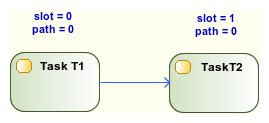
\includegraphics[width=\textwidth]{imgs/UML_SEQ_TSKS.png}
				\caption{Sequential tasks T1;T2.}
				\label{fig:UML_SEQ_TSKS}
        \end{subfigure}        
        \quad %\quad, \qquad, \hfill
        \begin{subfigure}[b]{0.4\textwidth}                
                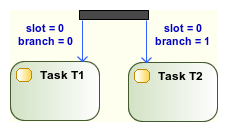
\includegraphics[width=0.8\textwidth]{imgs/UML_PAR_TSKS.png}
				\caption{Interleaved tasks T1\#T2.}
				\label{fig:UML_PAR_TSKS}
        \end{subfigure}%
          
\end{figure}

Sequential tasks ($T1;T2$) have subsequent time slots, meaning that T2's initial transition is synchronized to T1's final transition through PRISM labels. In contrast, interleaved tasks ($T1\#T2$) have their initial state transition synchronized at the same time slot through labels, but occupy different time paths, i.e., following state transitions of these tasks are interleaved.  Listings~\ref{lst:PRISM_SEQ_TSKS} and~\ref{lst:PRISM_INT_TSKS} present the DTMC modules for each case.
\medskip

\begin{lstlisting}[language=Prism, caption={Sequential tasks T15 and T16 as DTMC modules with final transitions of the first module synchronized to the initial transition of the former.},label={lst:PRISM_SEQ_TSKS}] 
const double rTaskT15=0.999;
module T15_LookupActiveSensors
	sT15 :[0..4] init 0;
	
	[success0_0]  sT15 = 0 -> (sT15'=1);//init to running	
	[] sT15 =  1 -> rTaskT15 : (sT15'=2) + (1 - rTaskT15) : (sT15'=4);//running to final state
	[success1_1] sT15 = 2 -> (sT15'=2);//final state success
	[success1_1] sT15 = 3 -> (sT15'=3);//final state skipped
	[failT15] sT15 = 4 -> (sT15'=4);//final state failure
endmodule

const double rTaskT16=0.999;

module T16_ReadActiveSensors
	sT16 :[0..4] init 0;
	
	[success1_1]  sT16 = 0 -> (sT16'=1);//init to running	
	[] sT16 =  1 -> rTaskT16 : (sT16'=2) + (1 - rTaskT16) : (sT16'=4);//running to final state
	[success1_2] sT16 = 2 -> (sT16'=2);//final state success
	[success1_2] sT16 = 3 -> (sT16'=3);//final state skipped
	[failT16] sT16 = 4 -> (sT16'=4);//final state failure
endmodule
\end{lstlisting}

\begin{lstlisting}[language=Prism, caption={Interleaved tasks T21.0 and T21.1 as DTMC modules with initial transition synchronized.},label={lst:PRISM_INT_TSKS}] 
const double rTaskT21_0=0.999;
module T21_0_DisplayEmergencyScreen
	sT21_0 :[0..4] init 0;
	
	[success0_2]  sT21_0 = 0 -> (sT21_0'=1);//init to running	
	[] sT21_0 =  1 -> rTaskT21_0 : (sT21_0'=2) + (1 - rTaskT21_0) : (sT21_0'=4);//running to final state
	[success1_3] sT21_0 = 2 -> (sT21_0'=2);//final state success
	[success1_3] sT21_0 = 3 -> (sT21_0'=3);//final state skipped
	[failT21_0] sT21_0 = 4 -> (sT21_0'=4);//final state failure
endmodule

const double rTaskT21_1=0.999;

module T21_1_CreatePlatformNotification
	sT21_1 :[0..4] init 0;
	
	[success0_2]  sT21_1 = 0 -> (sT21_1'=1);//init to running
	[] sT21_1 =  1 -> rTaskT21_1 : (sT21_1'=2) + (1 - rTaskT21_1) : (sT21_1'=4);//running to final state
	[success2_3] sT21_1 = 2 -> (sT21_1'=2);//final state success
	[success2_3] sT21_1 = 3 -> (sT21_1'=3);//final state skipped
	[failT21_1] sT21_1 = 4 -> (sT21_1'=4);//final state failure
endmodule
\end{lstlisting}

%Other supported behaviours are: alternative execution ($E1|E2$), optional execution (opt(E1)) and conditional execution (try(E)?E1:E2). For alternative execution,

\subsubsection{XOR-decomposition}

In the case of OR-decomposition with additional `|' behaviour rule, a resulting XOR-decomposition specifies that only one goal/task among two or more may be selected, i.e., they are mutually exclusive. Figures~\ref{fig:UML_ALT_TSKS} illustrate the alternative OR-decomposition in an UML activity diagram.

\begin{figure*}[ht!]
\centering
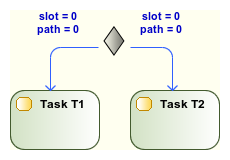
\includegraphics[width=0.35\textwidth]{imgs/UML_ALT_TSKS.png}
\caption{\detokenize{Alternative tasks T1|T2.}}
\label{fig:UML_ALT_TSKS}
\end{figure*}

To represent this rule in a DTMC model, an additional parameter  defines which alternative from a set of two or more is selected for analysis. Listing~\ref{lst:PRISM_ALT_TSKS} presents the DTMC modules for alternative tasks T9.00 and T9.01. For this behaviour rule, both time slot and time path are equal for the alternatives, as only one task may be selected. The increment is defined by surrounding `;' or `\#' rule. 
\medskip

\begin{lstlisting}[language=Prism, caption={Alternative tasks T9.00 and T9.01 as DTMC modules with additional integer parameter used for selection.},label={lst:PRISM_ALT_TSKS}] 
const double rTaskT9_0=0.999;
module T9_0_RESTRequisition
	sT9_0 :[0..4] init 0;
	
	[success0_2] (CONNECTION != 0) & sT9_0 = 0 -> (sT9_0'=1);//init to running
	[success0_2] !(CONNECTION != 0) & sT9_0 = 0 -> (sT9_0'=4);//init to failure
	[] sT9_0 =  1 -> rTaskT9_0 : (sT9_0'=2) + (1 - rTaskT9_0) : (sT9_0'=4);//running to final state
	[success2_3] sT9_0 = 2 -> (sT9_0'=2);//final state success
	[success2_3] sT9_0 = 3 -> (sT9_0'=3);//final state skipped
	[failT9_0] sT9_0 = 4 -> (sT9_0'=4);//final state failure
endmodule

const double rTaskT9_1=0.999;

module T9_1_SMSNotification
	sT9_1 :[0..4] init 0;
	
	[failT9_0]  sT9_1 = 0 -> (sT9_1'=1);//init to running
	[success2_3] sT9_1 = 0 -> (sT9_1'=3);//not used, skip running
	[] sT9_1 =  1 -> rTaskT9_1 : (sT9_1'=2) + (1 - rTaskT9_1) : (sT9_1'=4);//running to final state
	[success2_4] sT9_1 = 2 -> (sT9_1'=2);//final state success
	[success2_4] sT9_1 = 3 -> (sT9_1'=3);//final state skipped
	[failT9_1] sT9_1 = 4 -> (sT9_1'=4);//final state failure
endmodule
\end{lstlisting}

\subsubsection{Optional execution}

Given a decomposed goal or task, its fulfilment or execution may be optional, meaning that at least one other goal/task must necessarily be fulfilled/executed. It is trivial to realize that optional behaviour rules $opt(E)$ are only possible in OR-decompositions. Figure~\ref{fig:UML_OPT_TSK} illustrate an optional decomposition.

\begin{figure*}[ht!]
\centering
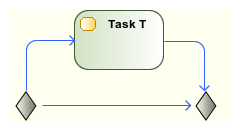
\includegraphics[width=0.37\textwidth]{imgs/UML_OPT_TSK.png}
\caption{\detokenize{Optional task T.}}
\label{fig:UML_OPT_TSK}
\end{figure*}

Similarly to alternative execution, optional tasks are enabled for analysis by an additional parameter in the model. Listing~\ref{lst:PRISM_OPT_TSK} illustrates the DTMC module for optional task T17.2. Time slot or path increment is also defined by surrounding `;' or `\#' rule. 
\medskip

\begin{lstlisting}[language=Prism, caption={An optional task T17.1 as a DTMC module with additional boolean parameter.},label={lst:PRISM_OPT_TSK}] 
const double rTaskT17_1=0.999;
const int OPT_T17_1;

module T17_1_PersistInDatabase
	sT17_1 :[0..4] init 0;
	
	[success1_3] (DISK <= 90) & sT17_1 = 0 -> (OPT_T17_1) : (sT17_1'=1) + (1 - OPT_T17_1) : (sT17_1'=3);//init to running or skip to final success
	[success1_3] !(DISK <= 90) & sT17_1 = 0 -> (sT17_1'=4);//init to fail
	[] sT17_1 =  1 -> rTaskT17_1 : (sT17_1'=2) + (1 - rTaskT17_1) : (sT17_1'=4);//running to final state
	[success1_4] sT17_1 = 2 -> (sT17_1'=2);//final state success
	[success1_4] sT17_1 = 3 -> (sT17_1'=3);//final state skipped
	[failT17_1] sT17_1 = 4 -> (sT17_1'=4);//final state failure
endmodule
\end{lstlisting}

\subsubsection{Conditional execution}

Some goals/tasks are conditioned to the fulfilment/execution of another goal/task. In such cases, a AND/OR-decomposition have an additional ternary rule $try(E1)?E2:E3$ where E2 is conditioned to the success of E1, while E3 is conditioned to its failure. The skip term is used if no further behaviour is conditioned to either the success or the failure of E1, for instance, in $try(T1)?skip:T2$ where task T2 is only required for execution if T1 fails and no further behaviour is expected if T1 succeeds. Figure~\ref{fig:UML_TRY_TSKS} illustrate a conditional decomposition.

\begin{figure*}[ht!]
\centering
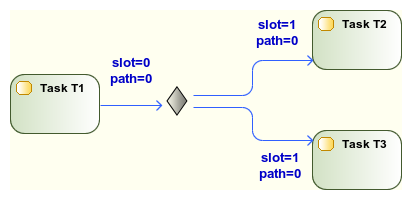
\includegraphics[width=0.60\textwidth]{imgs/UML_TRY_TSKS.png}
\caption{\detokenize{Optional task T.}}
\label{fig:UML_TRY_TSKS}
\end{figure*}

In conditional execution, labels are used to condition the execution of tasks to the success and failure of a third task. Figure~\ref{lst:PRISM_TRY_TSKS} present the DTMC module for conditional tasks T9.0 and T9.1. 
\medskip

\begin{lstlisting}[language=Prism, caption={Conditional tasks T9.00 and T9.1 as DTMC modules.},label={lst:PRISM_TRY_TSKS}] 
const double rTaskT9_0=0.999;

module T9_0_RESTRequisition
	sT9_0 :[0..4] init 0;
	
	[success0_2] (CONNECTION != 0) & sT9_0 = 0 -> (sT9_0'=1);//init to running
	[success0_2] !(CONNECTION != 0) & sT9_0 = 0 -> (sT9_0'=4);//init to failure
	[] sT9_0 =  1 -> rTaskT9_0 : (sT9_0'=2) + (1 - rTaskT9_0) : (sT9_0'=4);//running to final state
	[success2_3] sT9_0 = 2 -> (sT9_0'=2);//final state success
	[success2_3] sT9_0 = 3 -> (sT9_0'=3);//final state skipped
	[failT9_0] sT9_0 = 4 -> (sT9_0'=4);//final state failure
endmodule

const double rTaskT9_1=0.999;

module T9_1_SMSNotification
	sT9_1 :[0..4] init 0;
	
	[failT9_0]  sT9_1 = 0 -> (sT9_1'=1);//init to running
	[success2_3] sT9_1 = 0 -> (sT9_1'=3);//not used, skip running
	[] sT9_1 =  1 -> rTaskT9_1 : (sT9_1'=2) + (1 - rTaskT9_1) : (sT9_1'=4);//running to final state
	[success2_4] sT9_1 = 2 -> (sT9_1'=2);//final state success
	[success2_4] sT9_1 = 3 -> (sT9_1'=3);//final state skipped
	[failT9_1] sT9_1 = 4 -> (sT9_1'=4);//final state failure
endmodule
\end{lstlisting}


\subsubsection{Cardinality}

A small variation of the original RGM syntax was employed for the E+ and E\# rules. Instead of an undetermined number of goal/task instances, analyst should provide the exact number of instances for goals achievement and tasks execution. This information is required for the generation of the DTMC verification model from a runtime goal model. Figures~\ref{fig:UML_MUL_SEQ_TSKS} and \ref{fig:UML_MUL_PAR_TSKS} respectively illustrate sequential and interleaved task behaviours.

\begin{figure}[ht!]
        \centering
        \begin{subfigure}[b]{0.4\textwidth}
                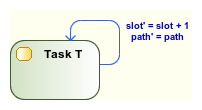
\includegraphics[width=0.80\textwidth]{imgs/UML_MUL_SEQ_TSKS.png}
				\caption{Sequential executions of task T.}
				\label{fig:UML_MUL_SEQ_TSKS}
        \end{subfigure}        
        \quad %\quad, \qquad, \hfill
        \begin{subfigure}[b]{0.4\textwidth}                
                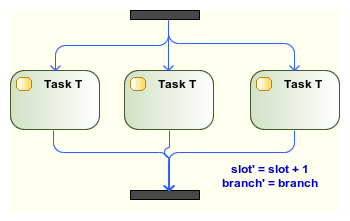
\includegraphics[width=0.80\textwidth]{imgs/UML_MUL_PAR_TSKS.png}
				\caption{Interleaved executions of task T.}
				\label{fig:UML_MUL_PAR_TSKS}
        \end{subfigure}%
          
\end{figure}

In our proposal, execution cardinality is represented by the number of retries of a given task transition from the initial state to the success state, in the case of a sequential execution ($E+n$), or by interleaved transitions with PRISM language module renaming, in the case of interleaved execution ($E\#n$). In the first case, only after $n$ unsuccessful retries, a transition to the failure state occurs. In the second case, $n$ simultaneous transitions from the initial state to the running state occurs before interleaved transitions from the running state to the final success/failure state may happen. The failure label is also renamed to avoid deadlocks if one or more of the interleaved tasks fails.

Despite the multiplicity of tasks instances, cardinality is seen as an execution block, i.e, the discrete time slot is only incremented once, while the time path is not incremented. Listings~\ref{lst:PRISM_MUL_SEQ_TSKS} and \ref{lst:PRISM_MUL_INT_TSKS} present the DTMC modules for both cases. The former example does not come from the MPERS RGM and illustrate the module renaming.
\medskip

\begin{lstlisting}[language=Prism, caption={Sequential cardinality with n=2 for task T22.},label={lst:PRISM_MUL_SEQ_TSKS}] 
const double rTaskT22;
const double maxRetriesT22=2;
module T22_ListenToButton
	sT22 :[0..4] init 0;
	triesT22 : [0..2] init 0;	
	
	[success0_3]  sT22 = 0 -> (sT22'=1);//init to running
	[] sT22 = 1 & triesT22 < maxRetriesT22 -> rTaskT22 : (sT22'=2) + (1 - rTaskT22) : (triesT22'=triesT22+1);//try
	[] sT22 = 1 & triesT22 = maxRetriesT22 -> (sT22'=4);//no more retries
	[success0_4] sT22 = 2 -> (sT22'=2);//final state success
	[success0_4] sT22 = 3 -> (sT22'=3);//final state skipped
	[failT22] sT22 = 4 -> (sT22'=4);//final state failure
endmodule
\end{lstlisting}
\medskip

\begin{lstlisting}[language=Prism, caption={Interleaved cardinality with n=3 for task T22.},label={lst:PRISM_MUL_INT_TSKS}] 
const double rTaskT22;
const double maxRetriesT22=2;
module T22_ListenToButton
	sT22 :[0..4] init 0;
	
	[success0_3]  sT22 = 0 -> (sT22'=1);//init to running
	[] sT22 = 1 -> rTaskT22 : (sT22'=2) + (1 - rTaskT22) : (sT22'=4);//running to final state
	[success0_4] sT22 = 2 -> (sT22'=2);//final state success
	[success0_4] sT22 = 3 -> (sT22'=3);//final state skipped
	[failT22] sT22 = 4 -> (sT22'=4);//final state failure
endmodule
module T22_N2 = T22_ListenToButton [ sT22_N2=sT22, rTaskT22_N2=rTaskT22 ] endmodule
module T22_N3 = T22_ListenToButton [ sT22_N3=sT22, rTaskT22_N3=rTaskT22, failT22_N2=failT22] endmodule
\end{lstlisting}

%Listing~\ref{ls:MPERS_DTMC} presents the DTMC model for the MPERS.

%To illustrate our proposal for NFR verification of a single alternative, we selected the local goal G5 that defines the state where emergency rules are updated without major system interruption. Table~\ref{tab:MPERS_NFR} has a non-functional constraint for this goal that specifies the minimum

In Table~\ref{tab:MPERS_DTMC_SLOTS}, the final settings for the time slot, path and other dynamic aspects of leaf-tasks parsed from the RGM and used for the generation of a DTMC model are presented.

% Please add the following required packages to your document preamble:
% \usepackage{booktabs}
\begin{table}
{\renewcommand{\arraystretch}{1.5}
\begin{tabularx}{\textwidth}{@{}lllllll@{}}
\toprule
\textbf{Task}  & \textbf{Time path} & \textbf{Time slot} & \textbf{Optional} & \textbf{Conditional} & \textbf{Alternative} & \textbf{Cardinality} \\ \midrule
\textbf{T15}   & 0                  & 0                  & false             & false                & false                & 1           \\
\textbf{T16}   & 0                  & 1                  & false             & false                & false                & 1           \\
\textbf{T17.0} & 0                  & 2                  & false             & false                & false                & 1           \\
\textbf{T17.1} & 0                  & 3                  & \textbf{true}    & false                 & false                & 1           \\
\textbf{T18}   & 0                  & 4                  & false             & false                & false                & 1           \\
\textbf{T19.0} & 0                  & 5                  & false             & false                & false                & 1           \\
\textbf{T19.1} & 0                  & 6                  & false             & false                & false                & 1           \\
\textbf{T20}   & 0                  & 7                  & false             & false                & false                & 1           \\
\textbf{T21.0}   & 1                & 7                  & false             & false                & false                & 1           \\
\textbf{T21.1}   & 2                & 7                  & false             & false                & false                & 1           \\
\textbf{T9.0}  & 3                  & 7                  & false             & false	        		& false                 & 1           \\
\textbf{T9.1}  & 3                  & 7                  & false             & \textbf{S. T9.0}     & false                 & 1           \\
\textbf{T22}   & 0                  & 8                  & false             & false                & \textbf{T24}                  & \textbf{2}  \\
\textbf{T23.0} & 0                  & 9                  & false             & false                & false                  & 1           \\
\textbf{T23.1} & 0                  & 9                  & false             & \textbf{S. T23.0}   & false                  & 1           \\
\textbf{T24}   & 0                  & 8                  & false             & false                & \textbf{T22}                  & 1           \\
\textbf{T25.0} & 0                  & 9                  & false             & false                & \textbf{T25.1                 } & 1           \\
\textbf{T25.1} & 0                  & 9                  & false             & false                & \textbf{T25.0}                  & 1           \\
\textbf{T5.0} & 4                   & 0                  & false             & false                & false                & 1           \\
\textbf{T5.1} & 4                   & 0                  & false             & false                & false                & 1           \\
\textbf{T5.2} & 4                   & 0                  & false             & false                & false                & 1           \\ \bottomrule
\end{tabularx}
\caption{Dynamic aspects of the MPERS leaf-tasks in the DTMC model.}
\label{tab:MPERS_DTMC_SLOTS}
}
\end{table}

\subsection{Context effects in the DTMC model}

In a CGM, the analysis of the environment in which the system will operate is performed. A careful investigation of what is static and what may change during operation should list the contexts facts and variables that may potentially affect goals, operational means (tasks) and the quality of alternatives. In contrast to the world predicates in the primitive CGM, in our proposal contexts are specified as boolean formulas composed of context variables and operators. Variables can hold boolean or real numbers values. The following operators can be used in the modelling environment:

\begin{itemize}

\item $<$, $<=$, $>=$, $>$ (relational operators)
\item $=$,\ $!=$ (equality operators)
\item $!$ (negation)
\item $\&$ (conjunction)
\item $|$ (disjunction)
%\item $-$ (unary minus)
%\item $*$, $/$ (multiplication, division)
%\item $+$, $-$ (addition, subtraction)

\end{itemize} 

Regarding a goal-oriented dependability analysis based on PMC, context variation may change the scope of the verification and consequently limiting the operational leaf-tasks that must be part of the analysis - either because they do not have a goal to satisfy in that context or because they are restricted by that context and cannot be selected for execution. Besides the effects over goals and tasks, we have not considered the direct context effect over qualitative softgoals, but only the indirect effect over the probability of fulfilling different system tasks, as softgoals are not part of the formal analysis.

All context effects formulas specified in the goal model are then parsed. Even if a context variable occurs multiple times in the same context formula or across other contexts in the model, only one variable is declared in the DTMC model (variable declaration). A reference to this variable is then used to compose identical context formulas as guard conditions in the modules corresponding to the affected leaf-tasks, according to the type of effect it imposes.

%and identical formulas are declared in the high-level DTMC model as guard conditions to the transition from the initial state to the running state

%In the DTMC verification model, context restrictions must follow a computable pattern. 

\subsubsection{Goals activation/restriction}

If a goal is activated/restricted by a given context selected for analysis, the corresponding verification scope must be adjusted. The MPERS RGM in Figure~\ref{fig:MPERS_LR} has a few goals whose activation depends on a specific context condition. Consequently, they must not affect the analysis results in other contexts.

For instance, the goals `stationary geolocation is checked' and `moving geolocation is tracked' are mandatory subgoals for the `patient location is monitored' goal. The first is activated by the context `user is at home' and the later by the negation of this same context. Analysts have put this restriction to avoid an aggressive geolocation tracking that consumes too much battery when the user is known to be at home. The following formulas specify this restricting context and its negation:

\begin{equation}\label{eq:C1a}
\textbf{C1:}\quad HOME\_WIFI\ !=\ 0\quad \&\quad LOCATION\_AGE\ <\ 10
\end{equation}

\begin{equation}\label{eq:C1b}
\textbf{!C1:}\quad HOME\_WIFI\ =\ 0\quad |\quad LOCATION\_AGE\ >=\ 10
\end{equation}

Home WI-FI BSSID is configured once and stored by the application. If its signal is not in reach for the last 10 minutes, patient is considered to be out. To map these restrictions into the DTMC model, only one PRISM formula were declared and all leaf-tasks related to the affected goals must include C1 (or its negation) as a condition to the inclusion of these tasks in the analysis. A false evaluation of the context formula (or its negation) automatically excludes these leaf-tasks from the analysis results by forcing a deterministic transition to the skipped final state (sTask=3). Listing~\ref{lst:PRISM_CTX_GOAL} presents the DTMC module of a MPERS leaf-task whose goal is restricted by a context formula.
\medskip

\begin{lstlisting}[language=Prism, caption={Variable declaration and corresponding module with a context activation formula.},label={lst:PRISM_CTX_GOAL}]
const double HOME_WIFI;
const double LOCATION_AGE;
const double rTaskT6_0=0.999;

module T6_0_CheckHomeWI_FIRange
	sT6_0 :[0..4] init 0;
	
	[success0_0] (HOME_WIFI != 0 & LOCATION_AGE < 10) & sT6_0 = 0 -> (sT6_0'=1);//init to running
	[success0_0] !(HOME_WIFI != 0 & LOCATION_AGE < 10) & sT6_0 = 0 -> (sT6_0'=3);//init to skipped


	[] sT6_0 =  1 -> rTaskT6_0 : (sT6_0'=2) + (1 - rTaskT6_0) : (sT6_0'=4);//running to final state
	[success0_1] sT6_0 = 2 -> (sT6_0'=2);//final state success
	[success0_1] sT6_0 = 3 -> (sT6_0'=3);//final state skipped
	[failT6_0] sT6_0 = 4 -> (sT6_0'=4);//final state failure
endmodule
\end{lstlisting}

\subsubsection{Tasks restriction}

Regarding the restriction on system tasks (means), all operations depending on a specific system resource considered to be dynamic could be notated with a context restriction. In our evaluation, we considered the restriction over the communication tasks `REST requisition' and `REST service' (context `internet is available'), over the geolocation tracking tasks `track public WI-FI' and `track GPS' (contexts `WI-FI is available' and `GPS signal is available') and over the storage task `persist in database' (context `disk memory available') . The following boolean formulas represent these contexts: 

\begin{equation}\label{eq:C2}
\textbf{C2:}\quad CONNECTION\ !=\ 0 
\end{equation}

\begin{equation}\label{eq:C3}
\textbf{C3:}\quad WI\_FI\ !=\ 0
\end{equation}

\begin{equation}\label{eq:C4}
\textbf{C4:}\quad GPS\_SIGNAL\ >\ 0
\end{equation}

\begin{equation}\label{eq:C5}
\textbf{C5:}\quad USED\_DISK <= 95
\end{equation}

These formulas follow the same principle from the previous goal restriction formulas. For C5, we considered less than 95\% of the used disk space and not 100\% to avoid instabilities in the operational system. We have not considered variations in the mobile signal as a restriction to the communication tasks of `SMS notification' and `voice call' or any other technical impediment at this moment. 

In the DTMC model, restricted leaf-tasks have an additional deterministic transition to the failure state guarded by the negation of the corresponding context formula. Consequently, if the formula is evaluated as false, the leaf-task will certainly fail (sTask=4). Listing~\ref{lst:PRISM_CTX_TASK} presents a DTMC model with one restricted MPERS leaf-task.
\medskip

\begin{lstlisting}[language=Prism, caption={Variable declaration and corresponding module with a context restriction formula.},label={lst:PRISM_CTX_TASK}] 
const double CONNECTION;//context variable declaration
const double rTaskT9_0=0.999;

module T9_0_RESTRequisition
	sT9_0 :[0..4] init 0;
	
	[success0_2] (CONNECTION != 0) & sT9_0 = 0 -> (sT9_0'=1);//init to running
	[success0_2] !(CONNECTION != 0) & sT9_0 = 0 -> (sT9_0'=4);//init to failure


	[] sT9_0 =  1 -> rTaskT9_0 : (sT9_0'=2) + (1 - rTaskT9_0) : (sT9_0'=4);//running to final state
	[success2_3] sT9_0 = 2 -> (sT9_0'=2);//final state success
	[success2_3] sT9_0 = 3 -> (sT9_0'=3);//final state skipped
	[failT9_0] sT9_0 = 4 -> (sT9_0'=4);//final state failure
endmodule
\end{lstlisting}

\section{Goal-oriented Reliability Analysis}

Once a probabilistic verification model is built from a system RGM with additional context effects, both qualitative and quantitative analysis may be performed. 

\subsection{Offline analysis}

%Formula verification consist of a qualitative or quantitative evaluation of a time-bounded or unbounded probability specified in PCTL language.

At design-time, analysts may benefit from the rich graphical environment provided by PRISM probabilistic model checker tool. Given a boolean formula specifying the success in fulfilling a specific system goal $G$ whose leaf-tasks have been mapped into the DTMC model:

\begin{equation}\label{eq:Gx}
G_{success}\ =\ (sT15=2)\ \&\ (sT16=2)\ \&\ (sT17\_0=2\ \&\ sT17\_1=2)
\end{equation}

And a PCTL property defining the probabilistic existence of a system behaviour that eventually leads the leaf-tasks T16, T17 and T17\_1 to reach their final success state, i.e., specifying the reachability of the success system state in which G is satisfied:

\begin{equation}\label{eq:PCTLx}
P > 0.99 [ F (G_{success})]
\end{equation}

Once the reliabilities of the involved leaf-tasks have been collected, the verification of this PCTL property through PRISM verification feature reveals the probability in eventually fulfilling the analysed goal. To illustrate this, for a fixed reliability of $0.98$ for rT15-17\_1, the reliability of $G$ is evaluated as $0.929199$. 

PRISM also provides the \textit{experiment} feature that automates multiple instances of a model checking. Instead of fixing the value of all variables in the model, one or more variables may range from a 

enables the evaluation of a given property considering fixed values and a range of values for different variables in the model. For instance, considering the same PCTL property~\eqref{eq:PCTLx}, an experiment  

%$G_{success}$ corresponds to MPERS goal `vital signs are monitored'. 

%one property may ask if the probability in fulfilling a given goal G is higher than P. 

\subsection{Gathering leaf-tasks reliabilities}

Leaf-tasks are not necessarily atomic system operations and are generally described with a high abstraction level. For instance, the MPERS task `Find active sensors' could be further decomposed in more granular and concrete tasks according to the platform, architecture and language used for implementation. 

%As presented in Figure~\ref{fig:MPERS_LR}, MPERS leaf-tasks are not coupled to any platform, architecture and language used for implementation.

%The idea is to leave to analysts the decision concerning the granularity and abstraction level represented by the tasks that will be verified. For instance, the abstract task `find active sensors' could be decomposed in more granular and concrete tasks related to the platform, architecture and language used for implementation. 

The more abstract a task is, the more difficult is to 
obtain their individual metrics - like their reliability, as the trace between an higher-level, abstract activity and the corresponding system operation(s) becomes less evident. For a global evaluation of a given metric, PCM technique requires the individual value for parts involved in the analysed system behaviour, e.g., activities, subactivities or components, depending on what the verification model represents.

In our goal-oriented approach, leaf-tasks are the parts composing a high-level system behaviour representation. Reliability variables define the probability of a successful execution of whatever the leaf-task should perform. To collect this information, analysts may follow two different approaches, as described in the next subsections. 

\subsubsection{Pure model-based verification}

A pure model-based verification 

\begin{figure*}[ht!]
\centering
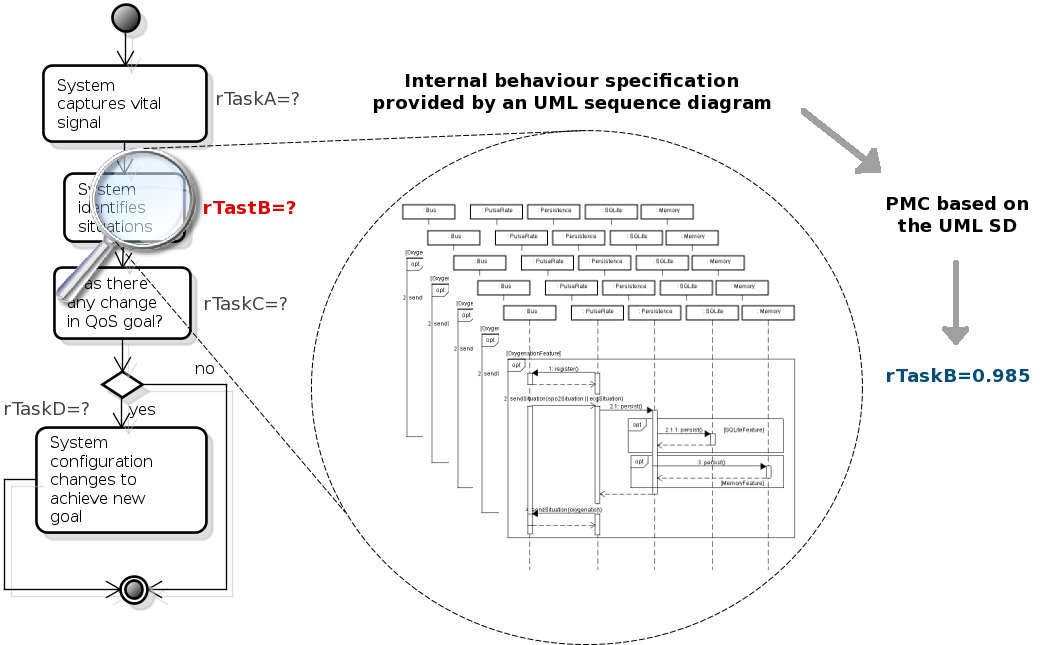
\includegraphics[width=0.75\textwidth]{imgs/MD_PMC.png}
\caption{Individual reliabilities of leaf-tasks are estimated through PMC of internal behaviour specification.}
\label{fig:MD_PMC}
\end{figure*}


. If internal behavioural specification like a sequence diagram is available for leaf-tasks, and if the reliabilities of the involved components are know, then a PMC approach can estimate the individual reliability of leaf-tasks. This value would then be used in the higher-level DTMC model. 

The original RGM proposal relies on a strong assumption that goals and tasks instance states can be monitored through some code instrumentation. Accordingly, the success rate of tasks execution, i.e., their reliability, can be extracted by monitoring the system execution trace in controlled executions or in real production environment. Figures~\ref{fig:MD_PMC} and~\ref{fig:MON_PMC} illustrate both approaches.

\subsubsection{Mean-time to failure verification}

and an hybrid approach based on the analysis of the monitored execution trace of system leaf-tasks.

\begin{figure*}[ht!]
\centering
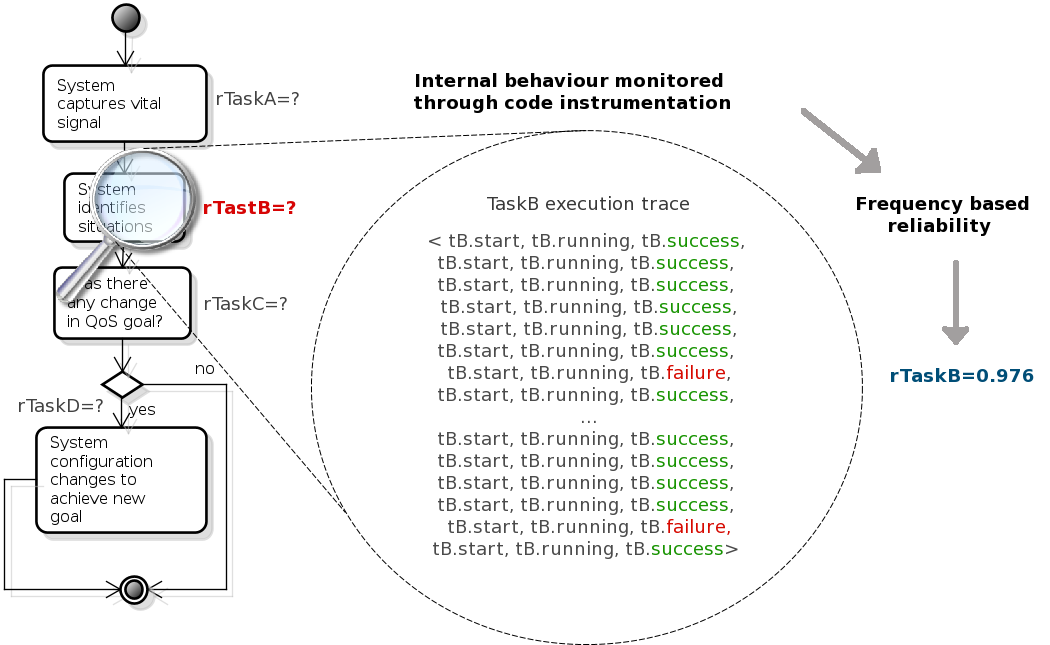
\includegraphics[width=0.75\textwidth]{imgs/MON_PMC.png}
\caption{Individual reliabilities of leaf-tasks are estimated by monitoring their execution.}
\label{fig:MON_PMC}
\end{figure*}


%In this work we focus on the creation of a parametric, high-level DTMC model corresponding to a runtime goal model with additional context effect notations to enable a goal-oriented reliability analysis for self-adaptive systems. 

As our proposal focus on the runtime reliability analysis for self-adaptive systems and monitoring is already part of a self-adaptation feedback loop, our evaluation with the MPERS case study is based on individual leaf-tasks reliabilities measured through instrumented code execution.

%Each NFR verified by the PMC technique requires corresponding information about individual parts involved in the overall activity, e.g., the reliability, performance, power consumption, cost and other metrics for tasks in a workflow.

%This is a key point in this approach, as it may seen too loose to couple a probabilistic verification to a goal model with a high-level operational representation of a system. But its feasibility becomes more clear if the metrics being verified are compatible with the abstraction level of the leaf-tasks in a specific goal model and individual task metrics are available or can be collected. 

%\subsubsection{Pure model-based approach}
%
%Depending on the purpose of the goal modelling - from early requirements elicitation to detailed design in TROPOS - more granular specification of tasks behaviour can be provided by decomposition and auxiliary UML diagrams. This internal task behaviour specification can be used for individual task analysis of metrics such as reliability and power consumption. 
%
%\subsubsection{Hybrid monitoring approach}
%
%In contrast to a pure model-based verification approach, the hybrid verification requires a concrete system implementation besides the RGM system model. Tasks execution instances could be monitored by instrumented code and the original RMG monitoring algorithms that are able to differentiate one task instance from the other. 
%
%In terms of reliability metric, this approach should be used to collect the frequencies of success and failure of task executions and to calculate their corresponding reliability values used in the high-level DTMC.

\subsection{Specifying non-functional constraints}

The specification of non-functional constraints is a sensible task that depends on both expertise and domain knowledge. For instance, an analyst or a reliability engineer should be aware of what does it mean for a system to be 99.99\% reliable, as this level may not be achieved by any alternative solution and must be coherent to the system criticality - a minor failure consequence could be tolerable, but a catastrophic failure should be avoided by all means. In some cases, the system will have to comply to some industry standards or contract based constraints like in service-oriented computing. Table~\ref{tab:MPERS_NFR} summarizes two possible non-functional constraints for the MPERS.
\medskip

% Please add the following required packages to your document preamble:
% \usepackage{booktabs}
\begin{table}[h]
{\renewcommand{\arraystretch}{1.5}
\begin{tabularx}{\textwidth}{@{}XXX@{}}
\toprule
\textbf{NFR}               & \textbf{Constraint} & \textbf{Target}        \\ \midrule
\textbf{Reliability}       & 99.8\%            & \textbf{G1} \\
\textbf{Power consumption} & 100 p.u.            & \textbf{G2}          \\ \bottomrule
\end{tabularx}
}
\caption{Non-functional metrics for the MPERS system.}
\label{tab:MPERS_NFR}
\end{table}

%softgoals of `continuous assistance' and `correct assistance'

As indicated by the \textit{Target} column, each NFR constraint may be associated to a root level goal or to any of its subgoals. The corresponding probabilistic verification based on the execution of a set of leaf-tasks in the RGM is defined as:

\begin{itemize}

\item \textit{Global}, if the activities set is a minimum set composed of the tasks that satisfies the chain of subgoals up to the root goal $Groot$. For instance, in Table~\ref{tab:MPERS_NFR} reliability is associated to root goal G1.
\medskip

\item \textit{Local}, if the activities set is a minimum set composed of tasks that satisfies the chain of subgoals up to a goal $Gx$, where $Gx != Groot$. For instance, in Table~\ref{tab:MPERS_NFR}, power consumption is (locally) associated to goal G2.
\medskip

\end{itemize}

%put here the formal definition of the root goal, subgoals, activity set, turple, etc

\subsection{From NFR to PCTL properties}

The estimation of attributes through PMC technique is limited to those that a probabilistic model may evaluate. Dependability attributes have an abstract definition that must be associated to a concrete and verifiable PCTL property. In this evaluation, we focus on the dependability attribute of reliability. 

Given a DTMC model representing system activities, global reliability may be defined as the probability of reaching a final state where all system goals are achieved. This property is called reachability and can be specified using the PCTL language. For the MPERS root goal G1, reliability can be defined by: $ P=? [ G (noError) ] $, with noError a boolean formula indicating that no task has transitioned to the failure state and P the steady-state probability of a true value for noError formula.


%\begin{itemize}
%
%\item \textbf{Reliability}, represented by the probability of a successful execution of all the activities involved in fulfilling leaf-goals of a certain system alternative. It is also know as the \textit{reachability} as the describes the probability of reaching a final and successful system state. 
%\bigskip
%
%\item \textbf{Availability}, represented by the power consumption estimation to maximize the time that the system will remain operational depending only on its battery. This attribute is well related to mobile computing. 
%\medskip
%
%\end{itemize}



%In Section~\ref{ssec:RGM-UML} we argued that the RGM could replace a corresponding high-level UML activity diagram for PMC verification. However, if internal task behaviour is to be evaluated for a given metric, a both activity and sequence diagrams could serve as input for the evaluation of individual task metrics using a similar PMC technique.

\subsection{Reasoning with Ex-Tropos}

The probabilistic verification of NFRs, performed as part of the Validation \& Verification (VV) phase in RE, should anticipate violations of non-functional constraints. Treating a detected violation at design time may correspond to actions such as making a different choice for underlying technical components or social actors involved in the execution of tasks, optimizing the behaviour specification or even disposing a violating alternative as a means to satisfy its goal if there is at least one other valid alternative. 

%PMC technique also allows the identification of system alternatives with more influence on each metric through sensitive analysis.

\subsubsection{Solving variability}

The variability in goal models leads to more than one minimum set of tasks capable of fulfilling local or root goals. In OR-decompositions, at least one alternative is required and the maximum number of combinations is defined by $1 + 2^{(n-1)}$, with n the number of OR-decomposed goals/tasks. Therefore, the verification of all alternatives in a goal model with individual models may prove to be inefficient or infeasible if too many variation points exist in the model.

The PMC approach has already been explored for the verification of other models that supports variability. Rodrigues et al. proposed a family-based verification of software product lines (SPL)~[RODRIGUES]. The main idea is to reduce the analysis effort and boost the feasibility of the SPL verification as parameters in a PRISM probabilistic model generates a single parametric formula for all products in the SPL for a given PCTL property. Individual product evaluation is achieved by the initialization of corresponding parameters in the formula. 

In our proposal, PCM verification follows the same principle of the SPL family-based verification. A parametric DTMC model should be generated from the runtime goal model. Alternatives are selected by passing values to parameters. For instance, if both GPS and triangulation are available means for identifying the patient location, a parameter with values 0 or 1 will indicate which alternative is enabled for verification, as described in Section~\ref{ssec:NFR-verification}.

\subsubsection{Context selection}

In a contextual goal model, or CGM, contexts may restrict which goals must be achieved, limit the adoptable alternatives (means) and also affect the non-functional metrics of individual tasks. These effects must be considered in a realistic verification. As a novelty, our approach for the verification of non-functional metrics through PMC will also include variable contexts of operation and their effects in the verification model. 

We considered two different approaches for the NFR verification of system with dynamic contexts of operation:

\begin{itemize}

\item \textit{Deterministic context activation, or DCA}: a single context is activated by parameters in the model. In this approach, a parametric formula evaluates a given alternative for a specific context of operation. It is useful for the individual verification of context-alternative pairs, e.g., a context where battery is fully charged and all vital signs sensors are activated.
\medskip

\item \textit{Probabilistic context selection, or PCA}: a probability distribution will define the likelihood of a context to be activated and the corresponding context implications in the verification model to be enabled. It is useful for the emulation of an approximate scenario in which the context of operation varies following some probabilist distribution. The resulting model evaluates an activated alternative for multiple contexts. 

\end{itemize}

Both approaches are complementary as the first verifies the selected alternative for one context at a time and the former verifies a realistic scenario with multiple possible contexts. Table~\ref{tab:SC_DCA_PCA} summarizes each verification approach.

% Please add the following required packages to your document preamble:
% \usepackage{booktabs}
\begin{table}[h]
{\renewcommand{\arraystretch}{2.5}
\begin{tabularx}{\textwidth}{@{}l|XX@{}}
\toprule
			 &                                                         \textbf{Context selection}			 &                                                                                                      \textbf{Alternative selection}			\\ \midrule
\textbf{DCS} & Contexts are individually activated by parameters.  & Alternative selection by the analyst is limited by the activated context.                                                                                    \\
\textbf{PCS} & Context selection follows a probabilistic distribution. & Verification model should select adoptable alternatives according to the activated context.\\ \bottomrule
\end{tabularx}
}
\caption{Description of the different approaches for verifying a system with variable alternatives and variable contexts.}
\label{tab:SC_DCA_PCA}
\end{table}

%If the context selection is deterministic (DCS), there is no reason for verifying an alternative that is known to be incompatible with the selected context. Therefore, only adoptable alternatives must be verified. In opposition, if context selection is probabilistic, that alternative may still be valid in other contexts, hence it must be included in the multi-context evaluation. For instance, the patient location identification through GPS (alternative) will certainly fail if the GPS signal is not available (context). Thus, the DAS-DCS combination checks one compatible context-alternative pair at a time, while DAS-PCS combination leads to the verification of multiple context-alternative pairs at the same time.

The idea behind a probabilistic context selection is to emulate a realistic scenario in which the context of operation varies and the system must avoid requirements violations by  having an adoptable alternative for each context. This holistic evaluation approach provides measures for the validation of self-adaptive systems against non-functional constraints like reliability.

weighted by the probabilistic context distribution. For instance, if GPS signal is available 70\% of the time and triangulation is available 90\% of the time and if each method has its own reliability, namely rGPS and rTRI, the reliability of high-level task `identify patient location' is defined by the expression 0.9*rGPS + 0.1*0.7*rTRI, considering that GPS has priority over triangulation. 

\section{Treating NFR Violations}

\begin{itemize}

\item Making a different choice for underlying components: In some cases the replacement of a technical component for another of the same class can improve the quality of how they achieve their goal. For instance,
\medskip

\item Behaviour optimization: The quality may also depend on the pattern used for the activities execution. The specification of a different pattern may eliminate the non-functional violation. 
\medskip

\item Contextualizing the alternative: An alternative may only violate a NFR in specific contexts. In this case, different valid alternatives may be used according to the context of operation.
\medskip

\item Alternative disposal: If the alternative is in absolute violation or if its validity is restricted to contexts that have at least one other valid alternative, this branch can be eliminated from the model.

\end{itemize}

%Dependability analysis is used to provide information about different dependability attributes related to system failures. These metrics may be specified as non-functional requirements for isolated system functionalities or for the whole system. Instead of softgoals, we use meta-requirements over functional goals with clear-cut quantitative criteria such as `99.999\%' reliable - a probabilistic value to make it compatible with the PMC estimation results.

%To perform the NFR verification, we focus on dependability related metrics that should be estimated and compared to their required constraint values through quantitative analysis. Sensitive analysis to reveal how different system parts contribute to the overall value of those attributes. Sensitive analysis may be considered analogous to the original GORE contribution analysis.



%Eq.~\ref{eq:MPERS_RELIABILITY_FORM} defines the reliability formula for the root goal G1.

%\begin{equation}
%G1r=c^2\label{eq:MPERS_RELIABILITY_FORM}
%\end{equation}

%A family-based PMC is useful for comparing each alternative with non-functional metrics as criteria to decide which one should be used by the system-to-be at design time or by the real system at runtime. At design time, this approach is analogue to the TROPOS contribution analysis. In both cases, a unique parametric formula evaluates a PCTL property corresponding to a non-functional metric.  %improve the example!


% or the verification tool should decide based on some probabilistic distribution setted by the analysts (probabilistic alternative selection, or PAS).

%In contrast, PAS provides verification for systems that include variability in its design. The verification of NFR metrics for these systems depend on how each alternative is selected during system operation.

